\documentclass[12pt,a4paper]{article}
\usepackage[utf8]{inputenc}%Entrada estándar
\usepackage[T1]{fontenc}
\usepackage[spanish]{babel} %Para usar palabras reservadas en Español
\deactivatequoting
\usepackage{amsmath} %Matemáticas
\usepackage{amsfonts}%Fuentes
\usepackage{amssymb}%Símbolos
\usepackage{xcolor} %Para colores
\usepackage{fancyhdr} %Para las cabeceras y pie de página
\usepackage[hidelinks]{hyperref}
\usepackage{parskip}%Para espacios en párrafos
\usepackage{float}%Para figuras, tablas, entre otros.
\usepackage{listings}%Para listas
\usepackage{subfigure} % subfiguras
\usepackage{epstopdf} %para irlo transformando a PDF
\usepackage{setspace}%Espacios...
\usepackage{filecontents} %Para las referencias
\usepackage{cite} %Para la cita
\usepackage{geometry}%Márgenes
%\usepackage[left=2.54cm, right=2.94cm, top=2.54cm, bottom=2.54cm]{geometry}%Márgenes APA
\usepackage{blindtext} %Para listas
\usepackage{enumitem} %Para enumerar listas
\usepackage{array}
\usepackage{graphicx}
\usepackage{fontawesome}

%%%% DEFINICIÓN DE COLORES %%%%%
\definecolor{verde}{rgb}{0.13, 0.55, 0.13} 
\definecolor{azul}{rgb}{0.17, 0.48, 0.69}
\definecolor{rojo}{rgb}{0.8, 0.0, 0.0}
\definecolor{amarillo}{rgb}{1.0, 0.88, 0.21}
\definecolor{ambar}{rgb}{1.0, 0.49, 0.0}
\definecolor{rojo2}{rgb}{0.83, 0.0, 0.0}
%%%%%%%%%%%%%%%%%%%%%%%%%%%%%%%%%

%%        DIVERSOS USOS       %%%
\geometry{margin=2cm}

\setlength{\headheight}{100.2pt} %Espacio en la cabecera
 %Estilo de la cabecera
\fancyhf{} %Limpiar el estilo predefinido de cabecera
\lhead{
\includegraphics[scale=0.085]{escudoUNAM}} %Cabecera imagen izquierda
\rhead{
\includegraphics[scale=0.14]{escudoFI}} %Cabecera imagen derecha
%\fancyhead[RO,LE]{\thepage}
\fancyfoot[C]{\thepage}
%%%%%%%%%%%%%%%%%%%%%%%%%%%%%%%%%%%%%%%%%%%%%

%Para nuestra tabla de contenidos o índice%
\setcounter{secnumdepth}{5}
\setcounter{tocdepth}{4}
%%%%%%%%%%%%%%%%%%%%%%%%%%%%%%%%%%%%%%%%%%
\pagestyle{fancy}
\begin{document}
	\newgeometry{left=2cm, right=2cm, top=1cm, bottom=2cm}
	\begin{titlepage}
	\begin{center}
		{ 
			\begin{tabular}{p{0.7\textwidth} p{0.50\textwidth} }
				
\includegraphics[scale=0.18]{escudoUNAM} &  
\includegraphics[scale=0.29]{escudoFI}
			\end{tabular}
		}
		
		\textcolor{azul}{\rule{\linewidth}{0.8mm}}\\
		\vfill
		{\LARGE \textbf{Universidad Nacional Autónoma de México}}
		\vfill
		{\LARGE \textbf{Facultad de Ingeniería}}
		\vfill
		{\Large {División de Ingeniería Eléctrica}}
		\vfill
		{\Large {Departamento de Ingeniería en Computación}}
		\vfill
		{\huge {Estructuras de Datos y Algoritmos II}}
		\vfill
		{\LARGE {Grupo 9}}
		\vfill
		{\LARGE {Tista García, Edgar}}
		\vfill
		{\LARGE {Proyecto \#2: Programación Paralela\\}}
		\vspace{3mm}
		{\LARGE {Semestre 2021-1}}
		\vfill
		{\Large {Equipo 11\\}}
		\vfill
		{\Large {Integrantes:\\}}
		\vspace{3mm}
		{\Large {Díaz Hernández, Marcos Bryan\\}}
		\vspace{3mm}
		{\Large {Lara Aguilar, Christian Abraham\\}}
		\vfill
		{\LARGE {20 de Enero de 2021}}
	\end{center}
\end{titlepage} %Incluimos la carátula al principio
	\restoregeometry
	\newgeometry{left=2cm, right=2cm, top=4.5cm, bottom=2cm}
	\renewcommand{\footrulewidth}{1pt}
	%-----------------------------------------------------
	%Índice
	\tableofcontents
	\vfill
	\clearpage
	%-----------------------------------------------------
	
	\section{Objetivo}
	Que el alumno implemente árboles binarios y que desarrolle sus habilidades la programación orientada a objetos a través de la aplicación del concepto de árboles como estructuras de datos no lineales
	
	\section{Introducción}
	Los árboles son estructuras que nos permiten modelar varios aspectos importantes de la vida diaria, como las operaciones, los sistemas de archivos, incluso modelos piramidales sencillos, ya que sus diferentes variantes pueden adaptarse a la necesidad. 
	
	En este proyecto se realizan las diferentes variaciones de un árbol binario: Heap, árbol de expresión y árbol binario de búsqueda binaria. Cada uno tiene sus propias formas de implementación y por medio de Java es posible realizar esta variaciones por medio de la herencia de las clases, además de implementar estas clases es necesario crear los métodos que cada uno de los árboles requiere para su correcta implementación.
	
	\section{Marco Teórico}
		\subsection{Árbol Binario}
	Antes de realizar los cada uno de los diversos tipos de árboles binarios que se requieren en el proyecto, hay que comenzar por definirlos. 
	
	Los arboles binarios son un tipo de árbol cuyos nodos pueden tener: cero, uno, o dos hijos. Para poder comprender mejor esta definición se conocen a los nodos de la izquierda de la raíz (nodo origen) como los hijos izquierdos y  a los nodos de la derecha de la raíz como hijos derechos. De igual forma se le conocen como subÁrboles a los hijos de la derecha e izquierda a partir de la raíz.

		\begin{figure}[h]
			\centering
			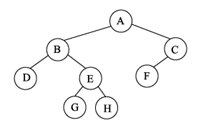
\includegraphics[scale=1]{ArbolB}
			\caption{Árbol Binario}
		\end{figure}

	Esta estructura se caracteriza por ser recursiva ya que cada nodo puede ser una raíz, y de esta forma tener subÁrboles a la derecha  e izquierda. Un elemento importante de los nodos es la altura de estos, que se define como el número de aristas que son necesarias para poder llegar al nodo hoja y el nivel en el cual se encuentran los nodos, que se define como la altura a la cual se encuentran todos los nodos, ya que estos datos permiten conocer cuál es el ultimo nodo y a que altura esta.

\begin{itemize}
\item Nodos hoja: Son aquellos nodos que se encuentran en la parte 			  inferior del árbol, es decir los últimos nodos que no tiene     	  hijos, de esta manera estos nodos indican la terminación del 		      árbol hasta ese punto donde se encuentren.
\item Nodos padre: Son los nodos que tiene uno o dos hijos, de tal       	  manera que se puede acceder a los hijos con la referencia que  		  tiene este sobre su hijo o hijos
\item Nodos raíz: Es el nodo principal a partir del cual se comienza 		  a construir un árbol, este es el único nodo que no tiene hijos. 
\end{itemize}

	En base a estas condiciones es posible establecer la estructura de un árbol binario:
	
El nodo esta compueso de dos o tres apuntadores de acuerdo a la version del árbol binario, debido a que incluso puede ser necesario tener una referencia del padre del nodo. Pero en condiciones normales es necesario tener dos referencias: nodo derecho, nodo izquierdo y un atributo que pueda contener informacion relativa a ese nodo.

		\begin{figure}[h]
			\centering
			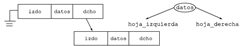
\includegraphics[scale=1]{Nodo}
			\caption{Nodo - Árbol Binario}
		\end{figure}
		
	Dentro de la estructura del arbol el conjunto de los nodos tienen referencias a sus hijos, derecho e izquierdo y contienen informacion que los distingue, el unico que no tiene padre es la raíz y en caso de que tuviera la referencia, esta sería nula.
	
		\begin{figure}[h]
			\centering
			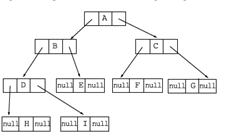
\includegraphics[scale=1]{ArbolBin}
			\caption{Árbol Binario Con Nodos}
		\end{figure}
	
		\subsection{Heap}

	El Heap es una variación del árbol binario, que tiene dos propiedades características: la primera corresponde al orden en que se deben colocar los nodos, de acuerdo con las reglas del Heap se debe conservar la integridad del árbol. Esto significa que se debe conservar a la raíz como el nodo con el valor mayor, y el cada nodo que sea padre deberá ser mayor a los nodos hijos. De tal manera que el recorrido del árbol desde la raíz hasta el ultimo nodo, ira en decremento del valor de los nodos.
	
		\begin{figure}[h]
			\centering
			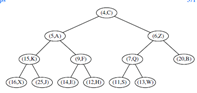
\includegraphics[scale=1]{Heap}
			\caption{Heap}
		\end{figure}

	De tal forma que después de cada inserción o eliminación se deba de comprobar esta condición por medio de los métodos que se encarguen de añadir o quitar elementos del Heap.
	
		\subsection{Árbol de expresión}
		
	El árbol de expresión se caracteriza por contener en lugar de enteros o valores numéricos, contener tokens, que expresen en operaciones algebraicas. Este cuenta con las siguientes características: 
	
\begin{itemize}
\item Cada hoja es un operando: suma, resta, multiplicación, 				  división.
\item Los nodos raíz y los nodos internos son operadores: 1,5,10,35.
\item Los subárboles son subexpresiones cuyo nodo raíz es un operador
\end{itemize}
		
		\begin{figure}[h]
			\centering
			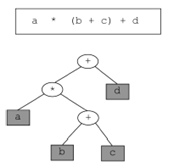
\includegraphics[scale=1]{ArbolExpre}
			\caption{Árbol de expresión}
		\end{figure}
		
	Las reglas para su construcción son:
	
\begin{enumerate}
\item Cada vez que se encuentra un paréntesis a la izquierda, se crea 	  un nodo que será la raíz, y será el nodo actual, después se 			  coloca en una pila. 
\item Cada vez que se encuentra un nuevo paréntesis a la izquierda, 		  se crea un nuevo nodo. Si el nodo actual no tiene hijo 				  izquierdo, este se convierte en su hijo izquierdo y si tiene 			  hijo izquierdo será entonces el hijo derecho. El nodo hijo será 	  el nuevo nodo actual y se coloca en la pila.
\item Cuando se encuentra un operando , se crea un nuevo nodo, se 			  asigna el operando al valor del nodo, y si el nodo actual no 			  tiene un hijo izquierdo el nodo nuevo se vuelve el hijo 				  izquierdo, en caso de que si lo tenga y no tenga derecho se 			  vuelve su hijo derecho.
\item Cuando se encuentra un operador, se saca de la pila el ultimo 		  elemento insertado y se colocar el operador en el campo del 			  nodo.
\item Ignorar el paréntesis derecho y blancos.
\end{enumerate}

		\subsection{Árbol binario de búsqueda equilibrado - AVL}
	Para esta variante es necesario el identificar las características de un árbol binario de búsqueda, el cual se caracteriza por tener un orden en la inserción de nodos y la eliminación de los nodos. Se denominan de esta manera ya que su estructura permite que sea posible buscar un elemento de igual forma que se puede en un arreglo ordenado.
	
	Su principal característica es que una vez definida la raíz, todos los nodos que pertenecen al subárbol derecho deberán ser mayores al valor del nodo raíz y los nodos que pertenecen al subárbol izquierdo deberán ser menores al valor del nodo raíz.
Debido a que son estructuras recursivas, esta condición se debe de cumplir para cada uno de los nodos internos, de tal forma que es un árbol ordenado. 

	Debido a esta misma condición la creación de los arboles resulta mas intuitiva ya que es similar a realizar un ordenamiento de los nodos, buscando donde corresponden de acuerdo con el valor que tengan.

		\begin{figure}[h]
			\centering
			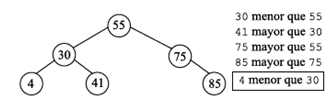
\includegraphics[scale=1]{ArbolBB}
			\caption{Árbol Binario de Búsqueda}
		\end{figure}

	La diferencia del árbol binario de búsqueda con el árbol binario de búsqueda equilibrado es  el valor de la altura de los subárboles, una vez que sabemos que es la altura del un árbol, podemos condicionar al árbol a que la diferencias de altura entre sus ramas no sea mayor a uno en altura. De tal manera que a esta altura limite se le conozca como un factor de equilibrio, con el cual se puede conocer cuantos nodos es posible agregar al subárbol derecho e izquierdo. 
	
	El factor de equilibrio puede tomar los valores: -1, 1, 0. De esta manera es posible que se limiten el añadir y eliminar. Al investigar se propone el uso de la expresión de Fibonacci, para poder determinar la altura máxima que puede tener un árbol y partir de esta determinar el factor de equilibrio de cada uno de los árboles.
	
	Como se mencionaba el añadir puede destruir el balance por ello se deben de implementar el rebalanceo del factor de equilibrio para el cual existen  cuatro casos para el proceso de inserción de un nuevo nodo. Los cuales son (I, I), (D, I), (I, D), (D, D). Para externos se utiliza la rotación simple y para los internos se utiliza la rotación doble.

	Para el caso de eliminar este proceso se realiza como le  método normal de la eliminación en arboles binarios de búsqueda, pero ahora se debe recorrer el árbol desde el nodo que se elimina hasta la raíz y actualizar los factores de equilibrio de los nodos y en caso de que se haya roto este balance se deberá de realizar una balance con la rotación simple o la rotación doble. 

		\begin{figure}[h]
			\centering
			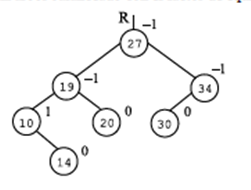
\includegraphics[scale=1]{ArbolE}
			\caption{Árbol Binario de Búsqueda Balanceado}
		\end{figure}


	\section{Análisis de las implementaciones}
		\subsection{Heap}

	La implementación de Heap, se lleva a cabo por medio de una ArrayList, mediante esta estructura es como pude implementar el Heap, esta forma fue una que vimos parcialmente en las clases, es una representación lineal debido a que utiliza una estructura lineal y no cíclica como un árbol.
	 
	Comenzando con el análisis de la clase el método constructor inicializa la lista que se utiliza para poder guardar los valores de los nodos.

		\begin{figure}[h]
			\centering
			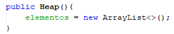
\includegraphics[scale=1]{MHeapA}
			\caption{Método Constructor}
		\end{figure}
		
	El método que permite la introducción de nuevos elementos a lista  los agrega a lista por medio del método add(), pero lo que realmente simula la implementación de un Heap es el método integridad padre e integridad hijo.

	El método IntegridadPadre() permite que se pueda comprobar la integridad del Heap por medio de la comprobación del valor del padre y del hijo. Al estar en una lista esta permite que se obtenga la posición de los valores al momento que se insertan, y por medio de las formulas para poder saber la posición del padre del ultimo nodo es posible realizar la comprobación de cuando se agrega un valor nuevo a la lista.

		\begin{figure}[h]
			\centering
			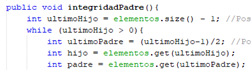
\includegraphics[scale=1]{MHeapB}
			\caption{Método integridadPadre() - 1}
		\end{figure}
	
	La siguiente condición del if, permite saber si el hijo es mayor al padre, y en caso de que se cumpla la condición se hace el intercambio de las posiciones, y ahora la posición del hijo pasa a ser la posición del padre, para que se pueda comprobar de nuevo con el nodo que tenía como hijo al padre del ultimo nodo insertado. De tal manera que se repita el proceso hasta que el hijo sea menor al padre.
	
		\begin{figure}[h]
			\centering
			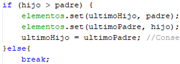
\includegraphics[scale=1]{MHeapC}
			\caption{Método integridadPadre() - 2}
		\end{figure}
	
	En el caso de la eliminación de eliminación de la raíz, se realiza el método eliminar() que se encarga de comprobar si existen valores en la lista y si se cumple la condición de que existan mínimo dos elementos en la lista se deberá de eliminar la raíz sustituyendo el valor de esta con el valor del ultimo hijo insertado.
	
	El método integridadHijo(), permite que se compruebe la integridad una vez se ha eliminado la raíz, de esta manera se comprueba que el valor de la raíz sea mayor a sus hijos, de esta manera es que se debe de comprobar que los hijos sean  menores, por lo que se debe comprobar con el hijo  izquierdo y el hijo derecho, el que sea mayor de ambos, será con el cual se comprobara la raíz para verificar la integridad


		\begin{figure}[h]
			\centering
			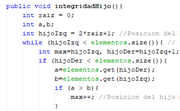
\includegraphics[scale=1]{MHeapD}
			\caption{Método integridadHjo() - 1}
		\end{figure}
		
	La segunda parte del  método es básicamente lo mismo que el método de IntegridadPadre(), debido a que si se cumple la condición de que el hijo sea mayor, se hace el intercambio de las posiciones y se vuelve a comprobar si los demás nodos son mayores al nuevo hijo que antes era la raíz. 
	
		\begin{figure}[h]
			\centering
			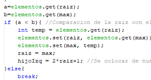
\includegraphics[scale=1]{MHeapE}
			\caption{Método integridadHjo() - 2}
		\end{figure}
		
		\subsection{Árbol de Expresión}
		
	La implementación de esta variante, esta fragmentada en varias clases, donde primero comenzare con ArbolExpre(), la clase tiene como atributo a una instancia de la case Solución(), mediante la cual es posible resolver la expresión que se transforma a PostOrden, de esta manera es posible que se tenga acceso al atributo de la clase Conversión().
	
	Es posible acceder a una tercera clase debido a que Solución() hereda de Conversión() entonces   a partir de la instancia que se tiene en la clase de ArbolExpre() es posible el tener acceso a los atributos de una tercera clase y ejecutar sus métodos desde Solución().
	
	Teniendo un poco mas claro de como se enlazan las clases, en la clase del árbol se lleva a cabo la implementación del método crearÁrbol(),  partir de la expresión que se convierte en PostOrden(). Entonces primero voy a analizar la clase que transforma y secuencialmente iré mostrando como van interactuando las clases.

			\subsubsection{Conversión}
			
	La clase conversión permite transforma la expresión, mediante el método conversionPost(), se transforma la cadena, primero se toma a la cadena como un conjunto de caracteres, y se va iterando uno a uno en un for de esta manera se puede comprobar la condición de cada uno de estos, ya sea paréntesis que abre, paréntesis que cierra, operando u operador.

En el caso de que sea un paréntesis de apertura, se mete a una pila, en caso de que sea un operando se concatena a una cadena Post que esta como atributo de la clase, en caso de que sea un operador de igual forma se envía a la pila. Para poder diferenciar entre un operador y un operando se envía el carácter a la función jerarquía que solo devuelve un entero mayor a 0 si es un operador el carácter enviado.

		\begin{figure}[h]
			\centering
			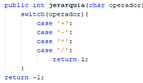
\includegraphics[scale=1]{MConversionA}
			\caption{Método Jerarquia()}
		\end{figure}
		
	Para el caso de los paréntesis que cierran, si se encuentra uno, esto significa que se ha finalizado un operación, esto es debido a la forma en que se deben de insertar las expresiones. Cuando se encuentra se comienzan a sacar los operadores de la pila hasta encontrar un  paréntesis de apertura que indique que el operador corresponde a esa primer cantidad de operandos que se han concatenado a la cadena atributo.
		
			\subsubsection{Árbol de Expresión}
	Una vez se ha transformado la cadena en PostOrden, esta se guarda en el atributo de la clase, y para esto se tiene la herencia de Solución() para poder acceder a la cadena y comenzar a crear el árbol. Para poder crear el árbol de expresión únicamente se necesita una pila, y se comienzan a seguir los pasos de la investigación, pero como la expresión ya no tiene paréntesis y esta ordenada, solo se verifican los operandos y  los operadores.
	
	Se repite el proceso de recorrer carácter por carácter la cadena y cada vez que se encuentre un carácter se deberá de introducir a la pila, pero ahora ese carácter esta dentro del atributo del nodo de esta forma en la pila se introducen nodos a la pila y se comienza a realizar el árbol. Continuando con la lógica de la construcción en caso de que se encuentre un operador este sacara a los nodos que contienen el valor de los operandos y los hará sus hijos derecho e izquierdo. Y se volverá a meter ese nodo a la pila para que el proceso se repita, de tal manera que la pila solo contendrá un nodo y este contendrá todo el árbol.
	
	Como la pila contiene solo un nodo, la raíz recibe este y se asigna a esta todo el árbol generado de la expresión. 

		\begin{figure}[h]
			\centering
			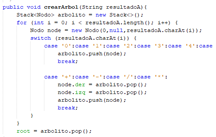
\includegraphics[scale=1]{MAExp}
			\caption{Método crearArbol()}
		\end{figure}
		
			\subsubsection{Solución}
	
	Una vez se tiene el árbol formado ahora se tiene que resolver la expresión,  mediante la instancia de solución se realiza el método resolver() que permite volver a leer la expresión carácter a carácter, y con una pila realizar la polaca inversa. Cuando se encuentra un operando este se coloca en la pila, y cuando se encuentra un operador, este saca a los valores de la pila para realizar la operación correspondiente. Una vez se realiza la operación se vuelve a colocar el resultado dentro de la pila.
	
	Este método es idéntico al método de creación de e los árboles, debido a que es prácticamente los mismo resolver la operación a representarla en un árbol en el caso de esta implementación ambos métodos realizan las mismas operaciones con su respectivo tipo de dato. Y como la pila conserva el valor del resultado este valor se regresa al atributo resultado que conserva el resultado hasta cuando sea solicitado por el usuario.

	\begin{figure}[h]
			\centering
			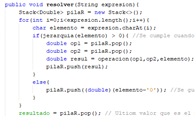
\includegraphics[scale=1]{MSolucion}
			\caption{Método Solucion()}
		\end{figure}
		
	\section{Conclusiones}
	Al realizar el proyecto parte por parte, me di cuenta de como se puede resolver un algoritmo por medio de la herencia y por la composición de las instancias, gracias al paradigma de orientado a objetos, y de igual forma note mis carencias en cuanto al paradigma, ya que algunos métodos no era necesario implementarlos o no era necesario realizar la herencia en ciertas clases. Pero por otro lado creo que lo que realice cumple con el objetivo del proyecto que es implementar las variantes de los arboles binarios, y por medio de la herencias es posible realizar esto, ya que cuando se tiene la base del árbol es necesario sobre escribir algunos métodos debido a que la variante es un especialización de la clase general.
	
Por ello considero que cumplí con comprender como realizar las distintas implementaciones aunque no hayan sido lo que se esperaba  o pedía, además el realizar un proyecto de forma individual me dejo un buen sabor de boca, y mas que nada desde el segundo proyecto mis ganas de hacer un proyecto por mi mismo fueron creciendo y  por eso decidí aventarme a realizar este proyecto de forma individual.

Gracias profesor.

	\section{Referencias Bibliográficas}
		\begin{thebibliography}{2}
			\bibitem{latexcompanion} 
			Joyanes L.. (2008). Estructuras de datos en Java. ESPAÑA: MCGRAW-HILL.
			
			\bibitem{knuthwebsite} 
			Michael T.. (2010). Data Structures and Algorithms in Java. United States of America: Wiley.
		\end{thebibliography}
	
	
	
	
	
	
	
	
	
	
\end{document}